\documentclass{beamer}

\mode<presentation>
{
  %\usetheme{CambridgeUS}
  \usefonttheme{professionalfonts}

  \usetheme{Singapore}
  \usecolortheme{orchid}
  %\setbeamercovered{transparent}
}

\usepackage{pgfpages}

\usepackage{verbatim,fancyvrb,times}
\usepackage{bm}
\usepackage[english]{babel}
\usepackage[utf8]{inputenc}
\usefonttheme[onlymath]{serif}
\usepackage[T1]{fontenc}
% Or whatever. Note that the encoding and the font should match. If T1
% does not look nice, try deleting the line with the fontenc.

\usepackage{amsmath}
\usepackage[amssymb]{SIunits}

\usepackage{hyperref}

\usepackage{tikz}
\usetikzlibrary{shapes,arrows,decorations.pathmorphing,calc}

\usetikzlibrary{shadows}
\definecolor{uaf red}{HTML}{E41A1C}
\definecolor{uaf blue}{HTML}{377EB8}
\definecolor{uaf green}{HTML}{4DAF4A}
\definecolor{uaf violet}{HTML}{984EA3}
\definecolor{uaf orange}{HTML}{FF7F00}
\setbeamercolor{boxed}{fg=black,bg=uaf yellow}

\newenvironment{transbox}{%

\begin{tikzpicture}
\node[drop shadow,rounded corners,text width=0.9\textwidth,fill=uaf violet, fill opacity=0.5,text opacity=1] \bgroup
}{
\egroup;\end{tikzpicture}} 

\newcommand{\Div}{\nabla\cdot}
\newcommand{\eps}{\epsilon}
\newcommand{\grad}{\nabla}
\newcommand{\lap}{\triangle}
\DeclareMathOperator{\trace}{tr}
\renewcommand{\bar}{\overline}

\newcommand{\ddx}[1]{\frac{\partial #1}{\partial x}}
\newcommand{\ddy}[1]{\frac{\partial #1}{\partial y}}

\newcommand {\jl}{[\![}
\newcommand {\jr}{]\!\hskip 0.003cm ]}
\newcommand{\bpsi}{\boldsymbol{\psi}}
\newcommand{\bPsi}{\boldsymbol{\Psi}}
\newcommand{\bphi}{\boldsymbol{\phi}}
\newcommand{\bPhi}{\boldsymbol{\Phi}}
\newcommand{\bn}{\mathbf{n}}
\newcommand{\bq}{\mathbf{q}}
\newcommand{\bv}{\mathbf{v}}
\newcommand{\D}{\,\mathrm{d}}
\newcommand{\Tsnow}{T_{\text{snow}}}


%\setbeamercolor{redtext}{fg=red!80!black}
\setbeamercolor{redtext}{fg=red!94!black}
%\setbeamercolor{greentext}{fg=green!80!black}
\setbeamercolor{greentext}{fg=green!60!black}
%\setbeamercolor{bluetext}{fg=blue!70!black}
\setbeamercolor{bluetext}{fg=blue!90!black}
\setbeamercolor{yellowtext}{fg=yellow!95!black}
\setbeamercolor{orangetext}{fg=yellow!50!red}

\newcommand{\green}{\usebeamercolor[fg]{greentext}}
\newcommand{\blue}{\usebeamercolor[fg]{bluetext}}
\newcommand{\red}{\usebeamercolor[fg]{redtext}}

\renewcommand{\L}{\emph{Left}}
\newcommand{\R}{\emph{Right}}



\title{generate pillboxes}

\author{Ed Bueler}

\institute{\tiny Dept of Mathematics and Statistics and Geophysical Institute \\
  University of Alaska Fairbanks}

\date{21 April, 2011}



\setbeamerfont{date}{size=\scriptsize}

%\begin{comment}
\AtBeginSection[]
{
  \begin{frame}<beamer>
    \frametitle{Outline}
    \tableofcontents[currentsection]
  \end{frame}
}
%\end{comment}

\begin{document}

\begin{frame}
  \titlepage
\end{frame}




\begin{frame}
  \frametitle{simple pillbox}

\begin{center}
        \begin{tikzpicture}[>=stealth,scale=1.75,decoration={random steps,segment length=3mm,amplitude=0.75mm}]
      \draw [decorate] (-2.5,0) .. controls (0,-.5) and (0,0.2) .. (2.5,0) node[anchor=west] {$\sigma$};
      \coordinate (A) at (0.03,-0.12);
      \coordinate [label=right:$w$] (B) at (-0.04,+0.25);
      \fill (A) circle (1pt);
      \draw[->] (A)  -- (B);
      \draw[rounded corners=1.5cm] (-2,-1) rectangle +(4,2);
      \node (plus) at (-1.25,0.75) {$V^{+}$};
      \node (minus) at (-1.25,-0.75) {$V^{-}$};
      \draw[->] (-.25,-1.25) node[anchor=north] {$\partial V$} -- (0,-1);
   \end{tikzpicture}

\end{center}

\end{frame}



\begin{frame}
  \frametitle{jump conditions across active layers include thin-layer transport}
\small

\begin{center}
        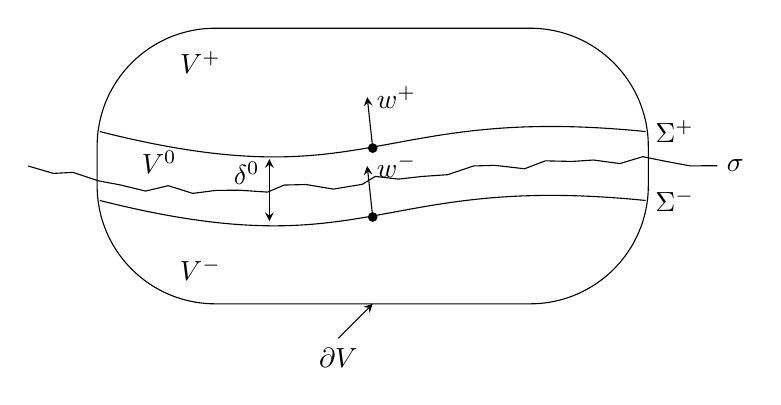
\begin{tikzpicture}[>=stealth,scale=1.75,decoration={random steps,segment length=3mm,amplitude=0.75mm}]
      \coordinate (U) at (-.75,0.05);
      \coordinate (D) at (-.75,-0.4);
      \coordinate [label=left:$\delta^{0}$] (delta) at (-.75,-0.05);
      \draw[<->] (U) -- (D);
      \draw [decorate] (-2.5,0) .. controls (0,-.5) and (0,0.2) .. (2.5,0) node[anchor=west] {$\sigma$};
      \foreach \ya / \side in {0.25/+,-0.25/-} {
        \coordinate (L) at (-1.98,\ya);
        \coordinate (R) at (1.98,\ya);
        \coordinate (CP1) at (0,\ya - 0.5);
        \coordinate (CP2) at (0,\ya + 0.2);
        \draw (L) .. controls (CP1) and (CP2) .. (R) node[anchor=west] {$\Sigma^{\side}$};
        \coordinate (A) at (0,\ya - 0.12);
        \coordinate [label=right:$w^{\side}$] (B) at (-0.04,\ya + 0.25);
        \fill (A) circle (1pt);
        \draw[->] (A)  -- (B);
      }
      \draw[rounded corners=1.5cm] (-2,-1) rectangle +(4,2);
      \node (plus) at (-1.25,0.75) {$V^{+}$};
      \node (zero) at (-1.55,0.03) {$V^{0}$};
      \node (minus) at (-1.25,-0.75) {$V^{-}$};
      \draw[->] (-.25,-1.25) node[anchor=north] {$\partial V$} -- (0,-1);
   \end{tikzpicture}

\end{center}

\end{frame}



\end{document}

